\documentclass[../main.tex]{subfiles}

\begin{document}
In questo capitolo si descrive la progettazione e lo sviluppo di una riproduzione del famoso gioco Snake adottando il paradigma Functional Reactive Programming. Al requisito non funzionale dell'utilizzo del paradigma FRP e del linguaggio di programmazione Scala si aggiunge anche quello dell'utilizzo della libreria \textit{Sodium}, analizzata nel capitolo precedente e scelta per la chiarezza e la completezza (ovvero il rispetto del paradigma FRP) delle API fornite.

I requisiti funzionali della applicazione \textit{FRP Snake} sono:
\begin{itemize}
    \item Il serpente si muove di una posizione nelle direzioni su, giu, destra e sinistra ed ha una dimensione iniziale pari a 1.
    \item Il numero di elementi che il serpente può mangiare è costante durante tutta la durata del gioco: quando il serpente mangia un elemento deve essere aggiunto un nuovo elemento.
    \item Gli elementi che il serpente può mangiare sono di due tipi: "buono", aumenta il punteggio complessivo di 100 punti e "cattivo", diminuisce il punteggio complessivo di 100 punti. In entrambi i casi il serpente aumenta la sua dimensione di 1 unità.
    \item La velocità di movimento del serpente è settata a 1 unità al secondo e può essere modificata a runtime in qualunque momento.
    \item Una partita si conclude quando il serpente è annodato.
\end{itemize}

\section{Progettazione}

\subsection{Input e Output}
\begin{figure}[H]
\centering
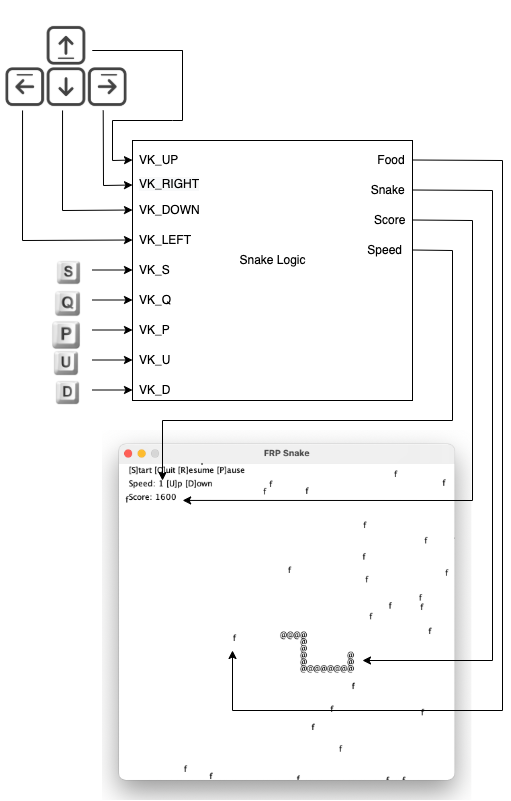
\includegraphics[width=0.9\textwidth]{img/frp-scala-Page-2.drawio.png}
\caption{Input/Output del programma FRP in relazione alla GUI}
\end{figure}

\begin{figure}[H]
\centering
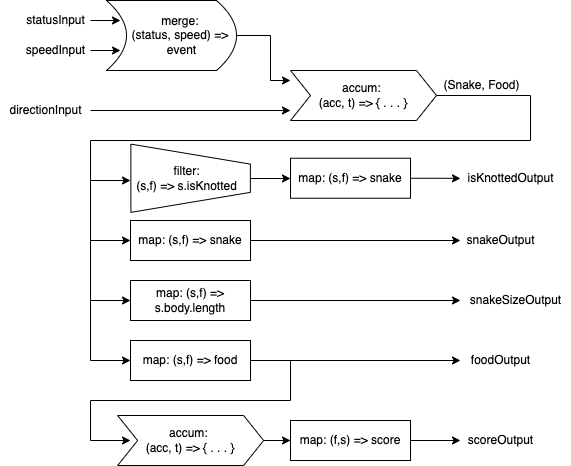
\includegraphics[width=0.9\textwidth]{img/frp-scala-Page-5.drawio.png}
\caption{Grafo delle dipendenze: FRP Snake}
\end{figure}
\end{document}

\section{Implementazione}
